\chapter{Theory Fundamentals}
Under the context of software engineering, a lot of effort have been spent in the scope of \textit{reuse}.
However most of the effort have been made code reuse, and not that much into software reuse as a whole.

In this chapter we provide the necessary definitions to understand \gls{FOP},
and how this paradigm copes with software reuse.
To simplify the understanding we will take the examples under software product lines.
This will also make clear how mechanizing a \gls{FOP} language shall benefit real world applications.


\section{Feature Oriented Programming}\label{seq:fop}

Feature-oriented programming (FOP) is a development approach 
that supports the \emph{stepwise refinement strategy} for software 
constructions~\cite{batory-tse2004}. Using FOP, a system is 
typically decomposed in (somewhat new) modular unities 
(named features) that resemble mixing layers~\cite{bracha-ecoop1990}, 
and thus are orthogonal to the typical object-oriented 
decomposition in terms of class hierarchies. 
Successful FOP usage scenarios have been reported in the literature 
for the domains of highly configurable systems and
software product lines~\cite{}.
FOP has been implemented using both programming 
language extensions and tooling support, such as 
Java AHEAD Tool Suite~\cite{batory_feature-oriented_2004} and \textsc{FeatureC++}~\cite{apel_featurec++:_2005}. 


\section{Software Product Line}
In the 70's the concept of software families was introduced by Parnas~\cite{parnas1976design}. 
It's main goal was to enhance the versatility to the development of the artefact's 
non-functional requirements. Upon this, the concept of \gls{SPL}
was formalized with the purpose of projecting several softwares
with similar characteristics under a single domain.

Sommerville\cite{Sommerville:2010:SE:1841764} defines\gls{SPL} as one of the most effective approaches to reuse.
And defines it as a set of applications with a common architecture and shared components.

As the name suggest, \gls{SPL} idea comes from Ford's product lines. With a product line
it is possible to build several different specializations of the same product, while
improving efficiency and reducing cost. This allow mass individualization of the products, i.e. even though the industry is still delivering products in mass scale,
it still provides somewhat individualized products for different kinds of clients.
The analogue still holds for \gls{SPL}, it proposes a framework which allows to build
several different specializations of the software, 
while reducing delivery time which by its turn reduces cost.

Take for example a \gls{SPL} illustrated in \ref{fig:cellphone-fm} for a mobile phone operational system. 
Every cellphone must be able to make calls and receive calls and having a screen. 
But there are optional features, such as having a GPS, being able to reproduce media,
etc.

\begin{wrapfigure}{r}{0.45\textwidth}
\centering
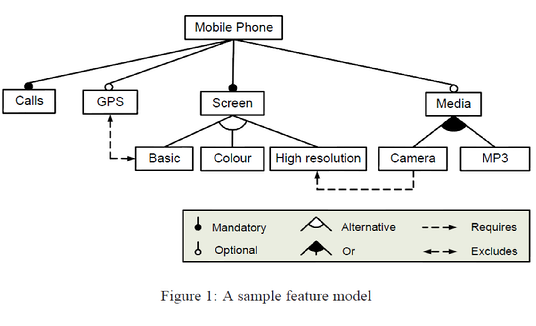
\includegraphics[scale=0.35]{doc/images/mobile-spl}
\label{fig:cellphone-fm}
\caption{Cellphone OS feature model} 
\end{wrapfigure} 

Formally a \gls{SPL} is defined by a triple: the \gls{FM}, \gls{CA},
and the \gls{CK}.

The \gls{FM} is the set of all features. They may be: \emph{obligatory}, \emph{optional}, \emph{alternative}, \emph{and} and \emp{or}.

The \gls{CA} is everything useful in the process of development, such as documentation, test cases, code, and so on.

The \gls{CK} is a mapping between features to assets, driving product generation.

With that in hand it is possible to compose the assets in order to provide a new product. However, it is not guaranteed that this composition process is safe, i.e.
that every asset selected copes well with each other. This leads us to the safe composition problem.

In order to tackle this safe composition problem, one could manually inspect
\gls{FM}, \gls{CK} and implementation to understand the dependencies between assets for all products. However, since \glspl{SPL} can quickly scale to hundreds of products,
this is often impractical.

Another approach would be to generate every single product, compile and test them.
While this is an useful and safe approach, it does not scale given the exponential 
factor in every feature introduction.

This is where formal methods shines. With formal methods it is possible to study how features interact with each other, postulate properties
and provide safety theorems for \glspl{SPL} without having to generate every single product.

\section{A Running Example: The Expression Product Line in \gls{FOP}}

\begin{wrapfigure}{r}{0.45\textwidth}
\centering
\includegraphics[scale=0.35]{doc/images/epl_fm}
\label{fig:epl_fm}
\caption{EPL feature model} 
\end{wrapfigure} 


In this section we illustrate the use of FOP through an AHEAD implementation 
of a slight adaptation of the Expression Product Line (EPL)~\cite{}---Figure~\ref{fig:epl_fm} shows 
the EPL feature model. Regarding our design decisions, 
in this case we implemented the mandatory features using a \textsc{base} AHEAD package (Figure~\ref{fig:epl-base}), which
declares a class hierarchy involving an interface (\texttt{Expression}) and
several classes (\texttt{Value}, \texttt{BinaryExpression}, \texttt{AddExpression}, and 
\texttt{SubExpression}), and one AHEAD package for each non-mandatory feature (see Figure~\ref{fig:epl-features}). Note 
that an AHEAD package contains either (a) plain Java entities (class or interface) declarations or (b) 
Java entities refinements. A refinement 
might override methods declared in other packages or 
introduce new attributes or methods in existing classes 
or interfaces. In this simple example, we do not implement any 
method overriding through class refinements---the refinements 
only introduce new elements to the \textsc{Base} AHEAD package 
of Figure~\ref{fig:epl-base}.  

\begin{figure}[htb]
\centering{
\includegraphics[scale=0.5]{doc/images/base.pdf}
}
\label{fig:epl-base}
\caption{The \textsc{base} package of the Expression Product Line}
\end{figure} 

The details of the EPL AHEAD non-mandatory feature packages are as follows. 

\begin{itemize}
\item Features \texttt{integer} and {double} refine the \texttt{Value} class of 
the \textsc{Base} package by introducing a new attribute named 
\texttt{value}, either with type \texttt{int} or \texttt{double}. According 
to the EPL feature model, only one of these features might be selected for 
a given product. 

\item The \texttt{expressions} feature introduces two new expressions 
to those declared in the \textsc{Base} package, one for multiplication 
and another for division. This particular feature does not refine 
existing classes, only introduces new ones. 

\item The \texttt{pretty\_printer} feature introduces the support for 
\emph{pretty printing} expressions. It refines the \texttt{Expression} 
interface and the \texttt{BinaryExpression} and \texttt{Value} classes, 
introducing a new method \texttt{print()} and also a 
new attribute (\texttt{operator}) for the \texttt{BinaryExpression} class.

\end{itemize}


\begin{figure}[htb]
\centering{
\includegraphics[scale=0.5]{doc/images/features.pdf}
}
\label{fig:epl-features}
\caption{Non-mandatory feature implementations of the Expression Product Line}
\end{figure} 

In the case we generate a product with  
a feature selection consisting of 
\texttt{EPL}, \texttt{value\_type(double)}, 
and \texttt{pretty\_printer}, we will get 
a product as shown in Figure~\ref{fig:epl-instance}. 


\section{Software Product line formal verification}